
\section{Translating Object Oriented Features Into \calculus}
\label{sct:scala-translation}
\usetikzlibrary{arrows, decorations.markings}
% for double arrows a la chef
% adapt line thickness and line width, if needed
\tikzstyle{vecArrow} = [thick, decoration={markings,mark=at position
   1 with {\arrow[semithick]{open triangle 60}}},
   double distance=1.4pt, shorten >= 5.5pt,
   preaction = {decorate},
   postaction = {draw,line width=1.4pt, white,shorten >= 4.5pt}]
\tikzstyle{innerWhite} = [semithick, white,line width=1.4pt, shorten >= 4.5pt]

\begin{figure}
\center
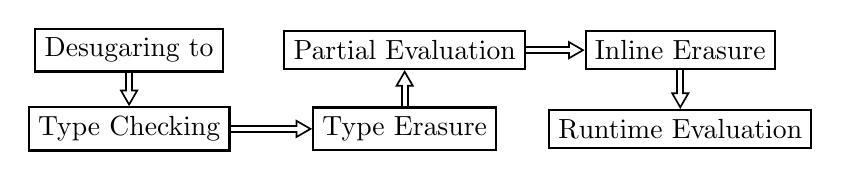
\begin{tikzpicture}[thick]
  \node[draw,rectangle] (a) {Desugaring to \calculus};
  \node[draw,rectangle,below of=a, node distance = 1.0cm] (b) {Type Checking \calculus};
  \node[draw,rectangle,right of=b, node distance = 3.5cm] (c) {Type Erasure};
  \node[draw,rectangle,right of=a, node distance = 3.5cm] (d) {Partial Evaluation};
  \node[draw,rectangle,right of=d, node distance = 3.5cm] (e) {Inline Erasure};
  \node[draw,rectangle,right of=c, node distance = 3.5cm] (f) {Runtime Evaluation};

  % 1st pass: draw arrows
  \draw[vecArrow] (a) to (b);
  \draw[vecArrow] (b) to (c);
  \draw[vecArrow] (c) to (d);
  \draw[vecArrow] (d) to (e);
  \draw[vecArrow] (e) to (f);

  % Note: If you have no branches, the 2nd pass is not needed
\end{tikzpicture}
\caption{Compilation pipeline.}
\label{fig:phases}
\end{figure}

% Description of the chapter

The core calculus \sct{sct:calculus} captures the essence of user-controlled
 predictable partial-evaluation. In practice, though, it requires an inconveniently large number
 of \code{inline} calls. Moreover, the calculus does not provide a way to define
 data structures that would correspond to \emph{classes} in modern multi-paradigm languages.
 In this section we formalize convenient implicit conversions for the calculus \sct{sct:conversions}, a scheme for
 translating classes into the calculus how to promote constructs classes and \emph{methods} into their
 partially-evaluated versions \sct{sct:promotion}.

% Restricted Language

The core rules of the calculus do not support effect-full computations and each
 \code{inline} term is trivially converted to a dynamic term after erasure.
 In case of languages that do support mutable state and side-effects this needs to
 be treated specially. For simplicity, we omit side-effects from our discussion and
 assume that all partially evaluated code is side-effect free and that each
 \code{inline} term can be converted to dynamic code.

\subsection{Desugaring Object Oriented Constructs to \calculus}
\label{sct:desugaring}

\begin{figure}
\begin{alignat*}{2}
   & [\![ \klet\ x: T_x = t_x\ \kin \ t ]\!] = ((x: T_x) \ra t)(t_x)\\
   & [\![ \klet\ type\ T_1 = T_2\ \kin\ t ]\!] =  ([T_1 <: T_2] \ra t)[T_2] \\
   & [\![ \klet\ class\ C[A](x: T_x) \{ def\ f[B](y: T_y) = t_f \}\ \kin\ t ]\!]  =  \\
   & \quad   \klet\ type\  C = [A] \ra \{ x: T_x, f: [B] \ra T_y \ra T_f \}\ \kin  \\
   & \quad \quad \klet\ C: [A] \ra (x: T_x) \ra C[A]  =  \\
   & \quad \quad \quad [A] \ra (x: T_x) \ra \{ x = x, f = [B] \ra (y: T_y) \ra t_f \}\ \kin\ t
\end{alignat*}
\caption{Desugaring of classes into \calculus.}
\label{fig:desugaring-classes}
\end{figure}

\subsection{Compile-Time View of Terms}
\label{sct:compile-views}
\begin{figure}
\begin{multicols}{2}[]

  \infrule[\textsc{CT-TVar}]
    {\Pi \ts T \in \Pi}
    {\Pi \ts \pe{iT}{iT}}

  \infrule[\textsc{CT-T-Var}]
    {\Pi \ts T \not\in \Pi}
    {\Pi \ts \pe{iT}{\inline{T}}}

\end{multicols}
\vspace{4pt}

  \infrule[\textsc{CT-Rec}]
    {\seq{\Pi \ts \pe{t}{t'}}}
    {\Pi \ts \pe{\i\{ \seq{x = t} \}}{\inline{\{ \seq{x = t'} \}}}}

  \infrule[\textsc{CT-T-Rec}]
    {\seq{\Pi \ts \pe{\i{T}}{\j{T}}}}
    {\Pi \ts \pe{\{\seq{x : \i{T}}\}}{\inline{\{ \seq{x : \j{T}}}\}}}

  \infrule[\textsc{CT-T-Arrow}]
    {\Pi \ts \pe{\i{T}}{\j{T}} \ \ \ \  \Pi \ts \pe{\k{S}}{\l{S}} }
    {\Pi \ts \pe{\i{T} \Rightarrow \k{S}}{\j{T} \Rightarrow \l{S}}}

  \infrule[\textsc{CT-T-Univ}]
    {\Pi \ts \pe{\j{T}}{\k{T}}}
    {\Pi \ts \pe{[X <: \i{S}] \ra \j{T}}{[X <: \i{S}] \ra \k{T}}}

  \infrule[\textsc{CT-Func}]
    {\Pi \ts \pe{t}{t'} \ \ \ \ \Pi \ts \pe{iT}{jT}}
    {\Pi \ts \pe{\i(x: iT) \ra t}{\inline{(x: jT) \ra t'}}}

  \infrule[\textsc{CT-TAbs}]
    {\Pi,\ X \ts \pe{t}{t'}}
    {\Pi \ts \pe{\i([X <: \j{T_1}] \ra t)}{\inline{([X <: \j{T_1}] \ra t'})}}

  \infrule[\textsc{CT-TApp}]
    {\Pi \ts \pe{t}{t'} \ \ \ \ \Pi \ts \pe{\i{T}}{\j{T}}}
    {\Pi \ts \pe{t[\i{T}]}{t'[\j{T}]}}

\caption{Translation of a regular class to a compile-time version.}
\label{fig:partial-evaluation}
\end{figure}
